\section{Introduction to boolean search}

The problem of boolean search is interesting, as this allows for answering queries of the type "List all articles that contain either shoe or boot and not sandal". In general, queries can be arbitrarily complex in terms of the nested structure of the boolean query. 

In order to search for such a boolean query, it needs to be represented in a structure that can easily be evaluated. A good choice for this is a syntax tree, from now on referred to as a \textit{Boolean query tree}. This contains the information of which words need to be looked up in the database, how the article lists need to be combined and in which order. All leaves in a boolean query tree consist of words. All parent nodes of a boolean query tree consist of a boolean operator. The depth, $d$, of a boolean query tree is defined as the maximum number of edges from the root node to a leaf. An example that has a depth of 2 is shown in figure \ref{fig:bool-st-example}.

\begin{figure}[ht!]
    \centering
    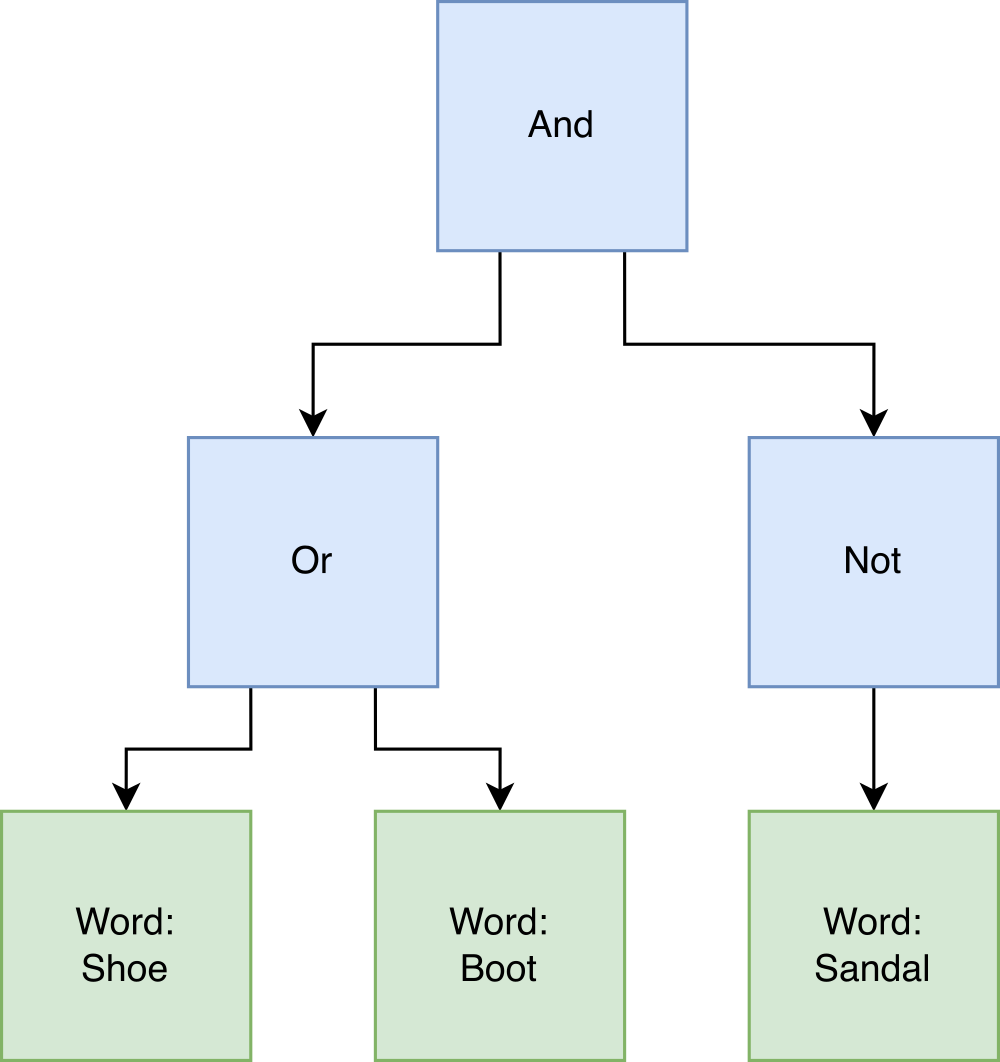
\includegraphics[width=.5\textwidth]{LaTeX/Figures/BooleanST.png}
    \caption{Example of a syntax tree for the query "(Shoe OR Boot) AND (NOT Sandal)"}
    \label{fig:bool-st-example}
\end{figure}

An important note about the NOT operation is that it only has one child in the boolean query tree, meaning that it reduces the branching (and thus the size) of the tree as a whole, as the size of the subtree below it is halved compared to the branching AND or OR operations. This makes analysing the size of a general tree and the complexity of algorithms on the tree a bit more tricky. For analysis, the worst case is usually when the tree is as large as possible, having $O(2^{d+1})$ nodes. 

When storing the information needed for these boolean queries and when evaluating these syntax trees, there are different approaches to how the data structures and algorithms are designed and which measures are prioritised. 

Index 7 and index 8 support Boolean search. The main difference is the data structure and how they store the list of articles that words appear in in the indices. Both of them use hash maps from a given word to the article list. 

\subsection{Reading and parsing user input}
To parse the user prompt into a boolean query tree code from \cite{parsing_lexing} was implemented. The user prompt is firstly lexed into boolean operators, after which the Boolean operators are parsed into an abstract syntax tree. The boolean operators "\&","," and "and" for the boolean AND operator, "|" and "or" for the boolean OR operator, and "!" for NEGATION is supported when lexing. The boolean operation NEGATION has the highest precedence whereas the AND and OR have equal precedence.\footnote{Contrary to normally, when AND has higher precedence than OR.} However, it is possible to use parentheses to specify the order in which the boolean operators should be evaluated. The user prompt "(shoe or boot) and not sandal" will thereby be evaluated in the order presented in figure \ref{fig:bool-st-example}.

